% Created 2019-01-24 Thu 13:56
% Intended LaTeX compiler: pdflatex
\documentclass[11pt]{article}
\usepackage[utf8]{inputenc}
\usepackage[T1]{fontenc}
\usepackage{graphicx}
\usepackage{grffile}
\usepackage{longtable}
\usepackage{wrapfig}
\usepackage{rotating}
\usepackage[normalem]{ulem}
\usepackage{amsmath}
\usepackage{textcomp}
\usepackage{amssymb}
\usepackage{capt-of}
\usepackage{hyperref}
\usepackage{minted}
\usepackage[margin=1.0in]{geometry}
\renewcommand\labelitemi{-}
\setlength{\parindent}{0pt}
\date{}
\title{Myths of Creation\\\medskip
\large Morford Chapter III}
\hypersetup{
 pdfauthor={Khayyam Saleem},
 pdftitle={Myths of Creation},
 pdfkeywords={},
 pdfsubject={},
 pdfcreator={Emacs 26.1 (Org mode 9.1.9)}, 
 pdflang={English}}
\begin{document}

\maketitle

\section*{Creation According to Hesiod}
\label{sec:org08455b5}
Hesiod (ca. 700) was the first to give literary expression to a systematic explanation of how the gods, the universe, and humankind came into being. This literary expression and geneaology is provided across \emph{Theogony} and \emph{Works and Days}.\\

In \emph{Theogony}, Hesiod discusses the beauty and power of the Muses. He discusses their ability to inspire the infallible revelations of the poet. He equates their inspiration and its fruits to prophecy.\\

He declares that before all came \textbf{Chaos}, a "yawning void." Birds are the oldest of all the Gods.
\begin{center}
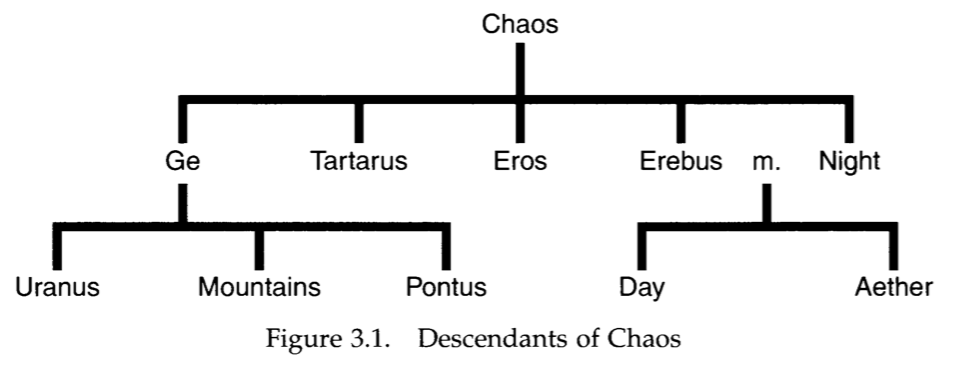
\includegraphics[width=250]{./descendants-of-chaos.png}
\end{center}

\section*{Creation According to Ovid}
\label{sec:org58a375e}
Ovid (ca. 1400) provides another classic account of genesis. Ovid's interpretation of \textbf{Chaos} differs from that of Hesiod in that rather than a gaping void, it is a crude and unformed mass of elements in strife from which a god or higher power formed the order of the universe. However, Ovid is Roman, and chronologically far removed from the origins of the mythology he professes.

\section*{Hesiod's \emph{Theogony}: The Sacred Marriage of Uranus and Gaia and Their Offspring}
\label{sec:org14c5336}
For Hesiod, the first deity is female. This matriarchical concept of mother earth and fertility corresponds well to divinity. Other primitive societies also agree upon the primacy of the feminine.\\

From here, the personification of Gaia as Earth and Uranus as Sky and their physical union provide a basis for a lot of the recurring themes in mythology. The rain of Uranus might be imagined as his seed that fertilizes the hungry Earth.

\begin{center}
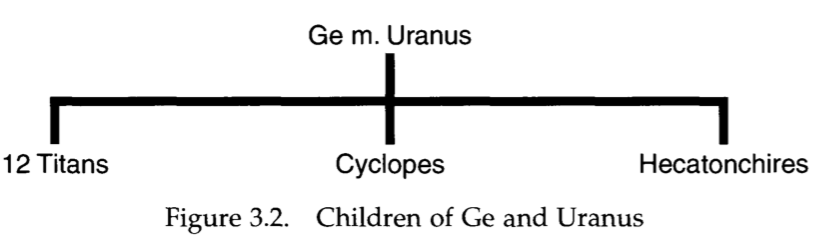
\includegraphics[width=250]{./children-of-ge-and-uranus.png}
\end{center}

\section*{The Titans and Their Descendants: Ocean, Sun, Moon, and Dawn}
\label{sec:orgea94816}

\begin{center}
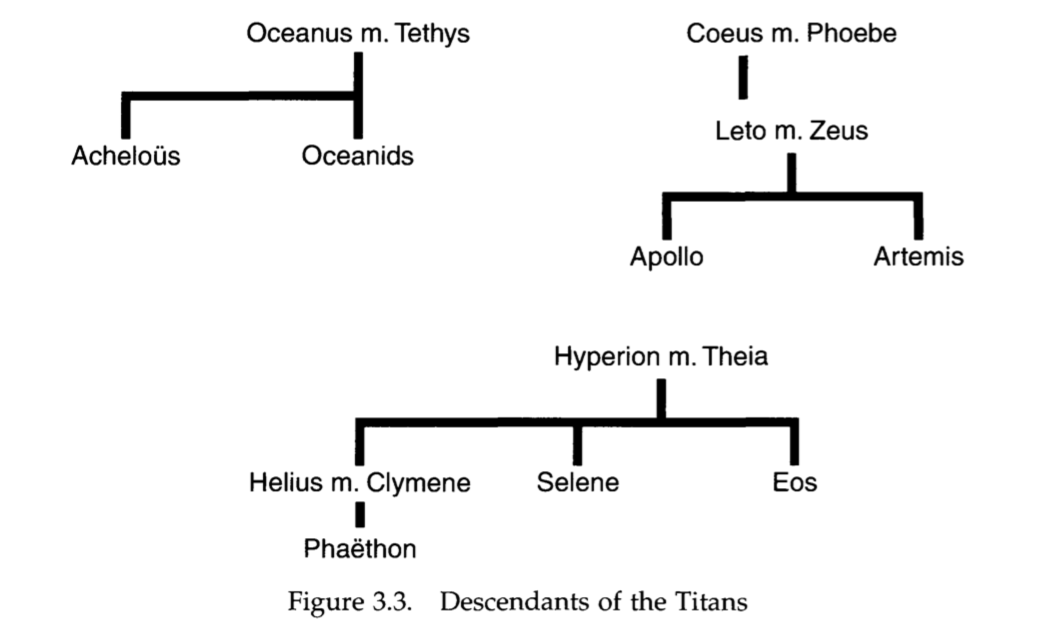
\includegraphics[width=250]{./descendants-of-the-titans.png}
\end{center}

There are 12 Titans: Oceanus, Coeus, Crius, Hyperion, Iapetus, Theia, Rhea, Themis, Mnemosyne, Phoebe, Tethys, and Cronus. They are deifications of various aspects of nature.\\

The Titans are best considered in pairs, as there are six males and six females, and they incestually produce cosmic progeny.
\end{document}
